\chapter{Numerical experiments and simulation results}

\begin{figure}[!htb] %Change this to [p] maybe ?
    \centering
    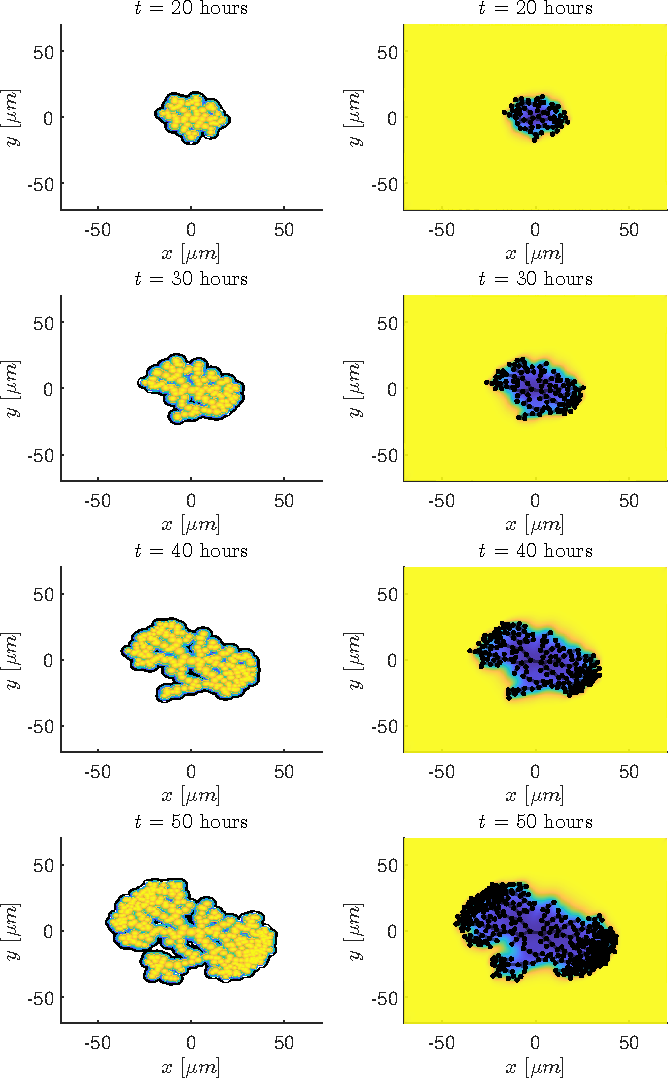
\includegraphics[width= 0.7\textwidth]{
        chapter2/figures/t_all__L1_0o10_L2_1o00_L3_1o00_L4_0o50_L5_1o00_L6_0o50_L7_1o00.pdf}
    \caption{A cell colony with parameter values given by
             $\lambda_1 = 0.1$,  
             $\lambda_2 = 1.0$, 
             $\lambda_3 = 1.0$, 
             $\lambda_4 = 0.5$, 
             $\lambda_5 = 1.0$, 
             $\lambda_6 = 0.5$, 
             $\lambda_7 = 1.0$. 
             On the left we have the biomass field, the nutrient field is on the right.}
    \label{fig: sdsd}
\end{figure}


\newpage


\begin{figure}[!htb] %Change this to [p] maybe ?
    \centering
    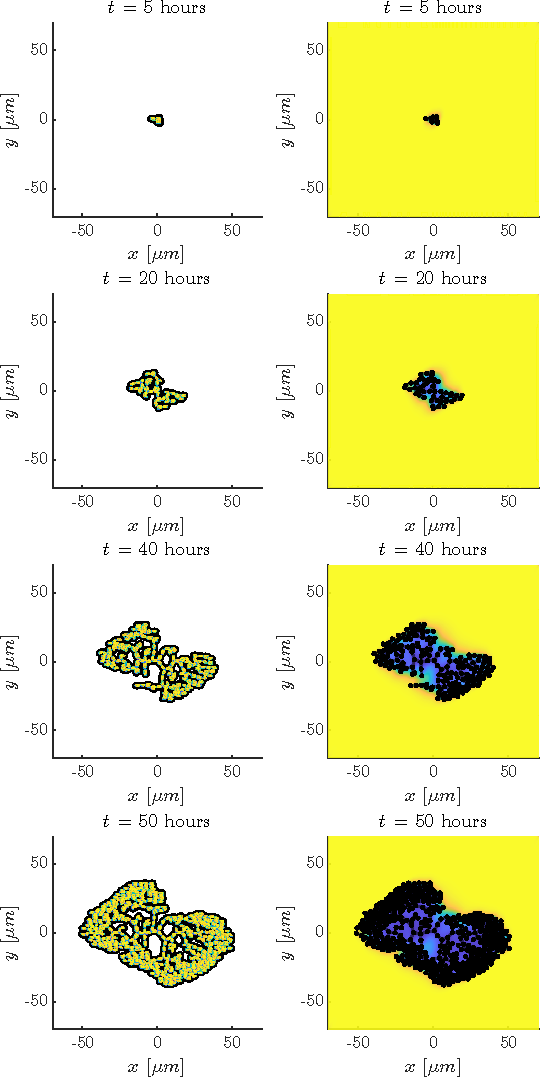
\includegraphics[width= 0.7\textwidth]{
        chapter2/figures/t_all_L1_0o10_L2_5o00_L3_1o00_L4_0o50_L5_1o00_L6_2o00_L7_0o50.pdf}
    \caption{A cell colony with parameter values given by
             $\lambda_1 = 0.1$,  
             $\lambda_2 = 5.0$, 
             $\lambda_3 = 1.0$, 
             $\lambda_4 = 0.5$, 
             $\lambda_5 = 1.0$, 
             $\lambda_6 = 2.0$, 
             $\lambda_7 = 0.5$. 
             Biomass on left and nutrient field on the right.}
    \label{fig: sdsd}
\end{figure}

\newpage

\begin{figure}[!htb] %Change this to [p] maybe ?
    \centering
    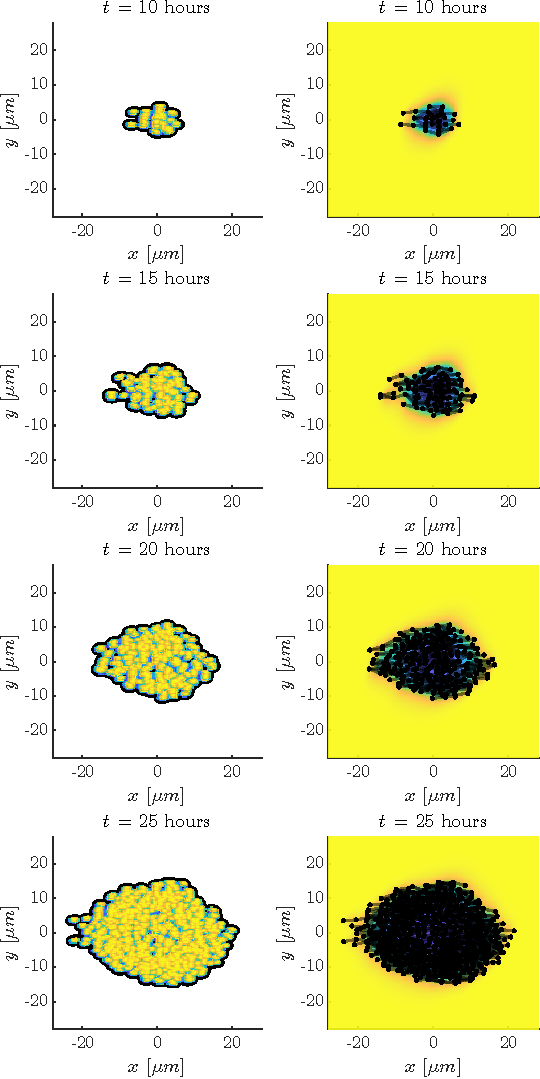
\includegraphics[width= 0.7\textwidth]{
        chapter2/figures/t_all__L1_0o10_L2_5o00_L3_1o00_L4_0o50_L5_1o00_L6_0o40_L7_0o60.pdf}
    \caption{A cell colony with parameter values given by
             $\lambda_1 = 0.1$,  
             $\lambda_2 = 5.0$, 
             $\lambda_3 = 1.0$, 
             $\lambda_4 = 0.5$, 
             $\lambda_5 = 1.0$, 
             $\lambda_6 = 0.4$, 
             $\lambda_7 = 0.6$. 
             Biomass on left and nutrient field on the right.}
    \label{fig: sdsd}
\end{figure}

\begin{figure}[!htb] %Change this to [p] maybe ?
    \centering
    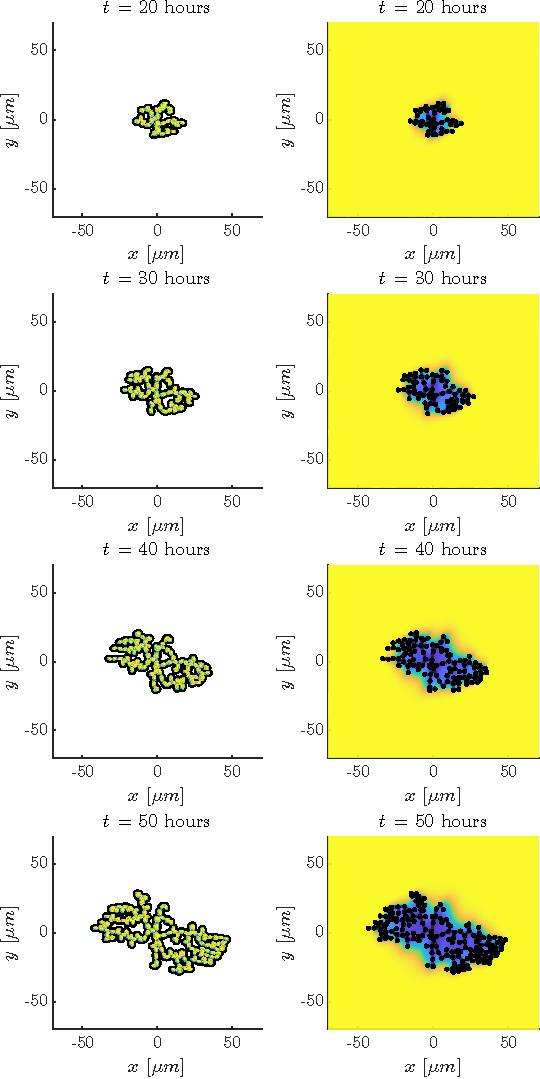
\includegraphics[width= 0.7\textwidth]{
        chapter2/figures/t_all__L1_0o10_L2_5o00_L3_1o00_L4_0o50_L5_1o00_L6_2o00_L7_0o60.pdf}
    \caption{A cell colony with parameter values given by
             $\lambda_1 = 0.1$,  
             $\lambda_2 = 5.0$, 
             $\lambda_3 = 1.0$, 
             $\lambda_4 = 0.5$, 
             $\lambda_5 = 1.0$, 
             $\lambda_6 = 2.0$, 
             $\lambda_7 = 0.6$. 
             Biomass on left and nutrient field on the right.}
    \label{fig: sdsd}
\end{figure}




\begin{figure}[!htb] %Change this to [p] maybe ?
    \centering
    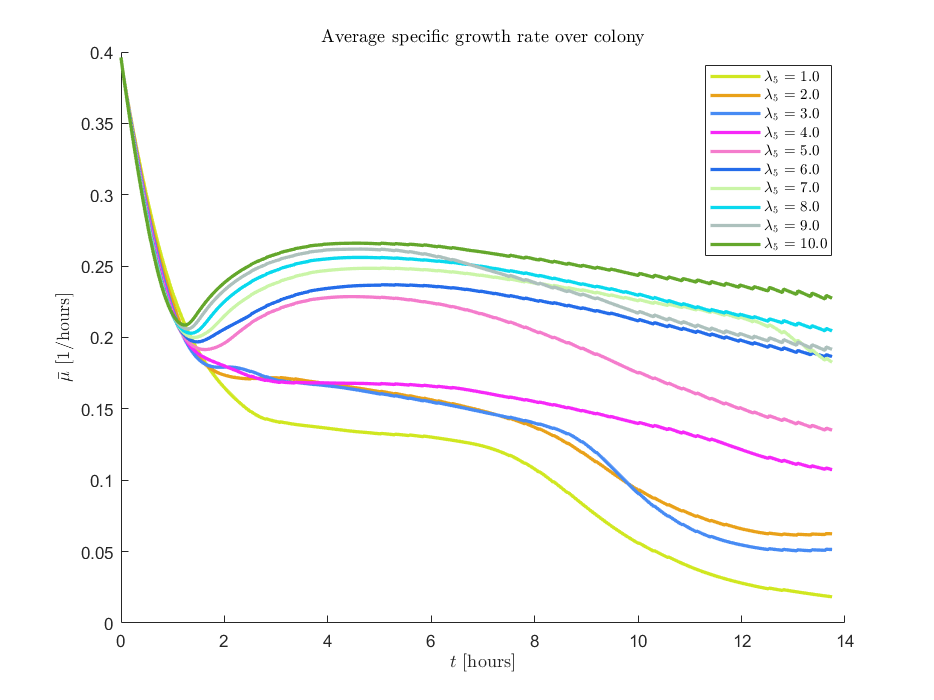
\includegraphics[width= 1\textwidth]{
        chapter2/figures/SpecificGrowthRatePlot.png}
    \caption{The colony average specific growth rate for different values of $\lambda_5$
                is measured and plotted over time for ensemble size $1$. The rest of the parameters 
                took the values:
                $\lambda_1 = 0.1$,  
                $\lambda_2 = 1.0$, 
                $\lambda_3 = 1.0$, 
                $\lambda_4 = 1.0$, 
                $\lambda_5$ (variable), 
                $\lambda_6 = 0.5$, 
                $\lambda_7 = 0.7$.
                Remarkably, when $\lambda_5 \geq 5.0$ there is an interesting dynamic that 
                occurs based on the compettition between nutrient consumption rate ($\lambda_6$)
                and the mobility ($\lambda_5$). For small values of mobility,
                the cells are not able to move enough into areas where the nutrient has not 
                decayed.}
    \label{fig:ColonySimulationNutrientFieldN210}
    \end{figure}
